% doc/tikz/launch_frame_chain.tex
\documentclass[tikz,border=5pt]{standalone}

\usepackage{amsmath, amssymb}
\usepackage{tikz}
\usetikzlibrary{
    arrows.meta,
    positioning,
    shapes.geometric,
    shapes.misc,
    calc
}

\begin{document}
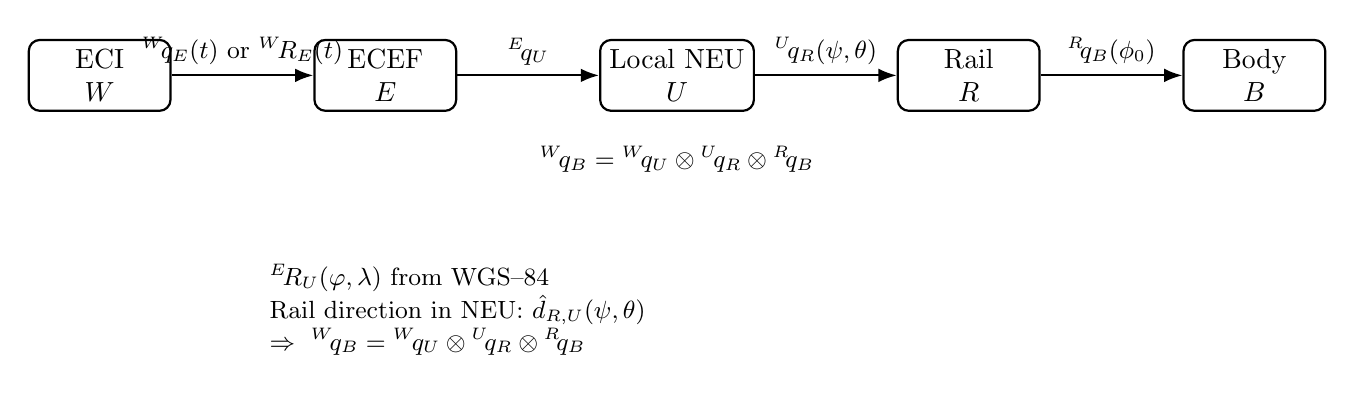
\begin{tikzpicture}[
    >=Latex,
    thick,
    frame/.style={rectangle, rounded corners, draw,
                  minimum width=1.8cm, minimum height=0.9cm,
                  align=center},
    axis/.style={->, very thick},
    lab/.style={font=\small}
]

% =========================
% 1) FRAME CHAIN (TOP)
% =========================
\node[frame] (W)                        {ECI \\ $W$};
\node[frame, right=1.8cm of W] (E)      {ECEF \\ $E$};
\node[frame, right=1.8cm of E] (U)      {Local NEU \\ $U$};
\node[frame, right=1.8cm of U] (R)      {Rail \\ $R$};
\node[frame, right=1.8cm of R] (B)      {Body \\ $B$};

\draw[->] (W) -- (E) node[midway, above, lab]
    {$^{W}\!q_{E}(t)$ or $^{W}\!R_{E}(t)$};
\draw[->] (E) -- (U) node[midway, above, lab]
    {$^{E}\!q_{U}$};
\draw[->] (U) -- (R) node[midway, above, lab]
    {$^{U}\!q_{R}(\psi,\theta)$};
\draw[->] (R) -- (B) node[midway, above, lab]
    {$^{R}\!q_{B}(\phi_0)$};

\node[below=0.3cm of U, lab]
    {$^{W}\!q_{B}
      = {}^{W}\!q_{U}\otimes{}^{U}\!q_{R}\otimes{}^{R}\!q_{B}$};

% Optional: small explanatory note
\node[lab, align=left] at (4.6,-3.0) {%
    \begin{tabular}{@{}l@{}}
      $^{E}\!R_{U}(\varphi,\lambda)$ from WGS--84 \\
      Rail direction in NEU: $\hat{d}_{R,U}(\psi,\theta)$ \\
      $\Rightarrow\ ^{W}\!q_{B}
        = {}^{W}\!q_{U}\otimes{}^{U}\!q_{R}\otimes{}^{R}\!q_{B}$
    \end{tabular}
};

\end{tikzpicture}
\end{document}
